\chapter{Preliminares}
\thispagestyle{empty}

\section{Introdução}


Neste capítulo fazemos uma revisão dos assuntos da matemática do ensino médio de que faremos uso ao longo do curso.
Apresentaremos de maneira rápida definições e alguns resultados básicos sobre números, funções com enfase nas funções lineares,
polinômios, exponecial e suas respectivas funções inversas. Posteriormente abordamos proporcionalidade,
 sistemas lineares e resolução de equações do segundo grau.

\section{Conjuntos Numéricos}

Os números são entidades abstratas usadas em processos que envolvem comparar quantidades, que se referem principalmente à contagem e medidas.
A habilidade de contar é considerada uma vantagem evolutiva, por exemplo para perceber quando há algum filhote faltando. De fato, são conhecidas diversas espécies,
além da humana,
com capacidade para distiguir pequenas quantidades. Em especial é notório que alguns corvos podem didtinguir quantidades que vão de um até seis.

Os números são o objeto central da matemática, e tem importância fundamental para diversas áreas do conhecimento que incluem finanças e econômia. Os conjuntos numericos pelos quais nos interessamos aqui são:
\begin{itemize}
\item[$\N$:] O conjunto dos \textit{números naturais}, são os números usados na contagem: $0,\,1,\,2,\,3,\,\ldots$ .
\item[$\Q$:] O conjunto dos \textit{números racionais}, são os números usados nas proporções. Os números
racionais são normalmente representados na forma de frações $\frac{1}{5}, \frac{2}{3}$, etc, ou na representação
decimal, por exemplo, $1,\,2,\,0,3333,\,\ldots$ . Todo número natural é também um número racional,
e admite representação como fração, por exemplo, $2=\frac{6}{3}$.
\item[$\R$:] O conjunto dos \textit{números reais}. É o conjunto usado em medidas de área,
comprimento, volume, etc. Os números reais são comunmente representados na forma decimal.
Todo número racional é também um número real.
\end{itemize}

Existem alguns tipos de operações que podemos fazer com estes conjuntos númericos, mais precisamente, soma, subtração, multiplicação e divisão. Considerando a natureza deste curso, não
nos ateremos nas operações com números. Admitiremos que os estudantes são proeficientes neste assunto.

\section{Intervalos}

Um intervalo $I$ é um subconjunto de $\R$ que satisfaz a seguinte condição:

\begin{mybox}
 Se $a$ pertence a $I$ e $b$ também pertence a $I$, sendo que $b>a$, então qualquer ponto intermediário $c$ (isto é, $a<c<b$) também pertence a $I$.
\end{mybox}

Um intervalo $I$ é \textit{fechado} se inclui suas duas extremidades. O intervalo I é \textit{aberto} se não inclui nenhuma das suas extremidades. Analogamente,
define-se intervalo \textit{aberto à direita} (fechado à esquerda) e intervalo \textit{aberto à esquerda} (fechado à direita).

\setlength{\parskip}{\baselineskip}\noindent\textbf{Notação:} Representamos um intervalo aberto pelas suas extremidades entre parenteses. Por exemplo, o intervalo aberto que compreende todos os números entre 2 e 5 é representado por $(2,5)$.
Representamos um intervalo fechado pelas suas extremidades entre parenteses. Por exemplo, o intervalo fechado que compreende todos os números de $\frac{3}{2}$ até $2$ é representado por $[\frac{3}{2},2]$.

\section{Funções}

Uma \textit{função} $f$ do conjunto $A$ para o conjunto $B$ é uma \textit{relação} entre os elementos de $A$ e de $B$, e esta relação deve satisfazer a seguinte condição:
\begin{mybox}
A função $f$ relaciona cada elemento $a$ do conjunto $A$ a um único elemento $b$ do conjunto $ B$. Denotaremos  $f(a)=b$.
\end{mybox}

\begin{exemplo} Abaixo um exemplo de uma relação que é função, pois satisfaz a condição acima, e outra que não é função.

\begin{multicols}{2}
\noindent \textbf{ É função:}
A relação que a cada número real associa seu quadrado $f(x)=x^2$
é uma função pois cada número real está associado a um único número real
que é seu quadrado.

\columnbreak

\noindent\textbf{ Não é função:}
A relação $\mathcal I$ que a cada pessoa associa um irmão ou irmã. De fato, algumas pessoas tem mais de um irmão ou irmã.

\end{multicols}


\end{exemplo}

O conjunto $A$  é chamado  \textit{domínio} de $f$ e o conjunto $B$ é chamado \textit{contra-domínio} de $f$.
Denotamos o domínio de $f$ por $\D(f)$.  Outro elemento importante no estudo de funções é
o conjunto
$$ \Im(f)=\{y\in B:\mbox{ existe algum }x\in A \mbox{ que satisfaz }f(x)=y\},$$
que é a \textit{imagem} de $f$.

Enquanto o contra-domínio $B$ pode se tratar de uma descrição vaga, que geralmente serve apenas para delimitar a natureza dos objetos
que são produzidos por uma função $f$, a imagem desta função contém apenas os elementos  que são de fato produzidos pela aplicação de $f$
ao conjunto $A$.

%\vspace{0.5cm}
\vfill
%\vspace{0.5cm}
\clearpage



% \begin{multicols}{2}
\begin{exemplo}
 Considere a função que $\zeta$ a cada elemento químico associa seu número atômico. Então o domínio de $\zeta$, $\D(\zeta)$,
 será o conjunto de todos os elementos químicos. O contra domínio de $\zeta$
será o conjunto $\N$ dos números naturais. A imagem de $\zeta$ será o conjunto dos números naturais que são o número atômico de algum elemento químico, isto é,
  são todos os números naturais de 1 até 118, ou seja $$\Im(\zeta)=\{1,2,3,4,\ldots,117,118\}$$

O elemento químico Hélio é tradicionalmente representado pela sigla He, e seu número atômico é 2.
Assim usando nossa notação matemática este fato é representado assim: $$\zeta(\mbox{He})=2.$$
\end{exemplo}


Neste curso tratamos apenas de funções
cujo domínio e o contra domínio são conjuntos numéricos, principalmente os números reais e intervalos de números reais. Quando a função relaciona conjuntos númericos
usualmente esta função é dada por uma ou mais fórmulas. Por exemplo, a função $f$ de $\R$ em $\R$ que pega um número real e retorna o triplo deste número, é dada pela fórmula
$f(x)=3x$.
% \columnbreak

\begin{tcolorbox}
% \begin{minipage}{7cm}
\noindent\textbf{ Hora do cafezinho:}
\begin{cursive}
A função $f$ de $A$ em $B$ pode ser imaginada como uma máquina que usa como matéria prima os elementos de $A$ e produz elementos de $B$.
Por exemplo, se $f$ é uma determinada máquina de café expresso de cápsula, cujo fabricante disponibiliza os segintes tipos de cápsulas:
$$A=\left\{ \begin{array}{c}\mbox{\small Grão Brasileiro, Grão Colombiano,}\\\mbox{\small Grão Baunilha, Grão Frutado,}\\\mbox{\small Grão Intenso}  \end{array}\right\}.$$
A cada tipo de cápsula $f$ associa um tipo de café.
O conjunto $A$ é o domínio de $f$.
O contra domínio será, digamos, o conjunto $B$ de todos os sabores de café que existem.
Porém a imagem, $\Im{f}$, é a coleçaão que contém apenas o sabores de café que saão de fato produzidos pela máquina, isto é,
$${\footnotesize \Im(f)=}\left\{\begin{array}{c}\mbox{Café sabor Brasileiro,}\\ \mbox{Café sabor Colombiano,}\\ \mbox{Café sabor Baunilha},\\ \mbox{Café sabor Frutado,}\\ \mbox{Café sabor Intenso}\end{array} \right\}.$$
\end{cursive}
% \end{minipage}
\end{tcolorbox}
% \end{multicols}

% \vspace{0.5cm}


\section{Gráfico de uma função}

Uma função $f$ com domínio e contradomínio em $\R$ pode ser representada de forma precisa por meio de uma figura que chamamos o \textit{gráfico de }$f$.
Antes de nos aprofundarmos no conceito de gráfico de uma função, precisamos definir o plano cartesiano.

%\vspace{0.5cm}

\noindent\textbf{Plano Cartesiano:} O plano cartesiano pode ser construído a partir de qualquer plano dado da seguinte forma:
Considere um plano $\mathcal{P}$.  Escolhemos de forma arbitrária um
ponto $O$ no plano $\mathcal{P}$, que chamaremos de \textit{origem}. A origem será nosso ponto de referência no planto $\mathcal{P}$.
Agora traçamos sobre $\mathcal{P}$ duas retas que se cruzam em $O$ e são perpendiculares entre si. Chamaremos estas retas de eixo $x$, e eixo $y$. Por convensão
o eixo $x$ é representado na horizontal e o eixo $y$ na vertical.

\begin{center}
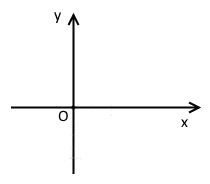
\includegraphics{./chapters/preliminares/imgs/Eixosxy}
\end{center}


Fixemos uma unidade de comprimento $u$ (pode ser cm, m,\ldots etc).
A partir daí  cada ponto do plano $\mathcal{P}$ é associado a um par ordenado de números $(x,y)$, da seguinte forma:
 O ponto $(x,y)$ é o ponto a que chegaremos partindo da origem $O$ e:


\begin{mybox}

\begin{itemize}
\item[$\bullet$] Caminhando
$x$ unidades $u$ para a direita se $x$ é positivo (ou  $-x\ u$ esquerda se $x$ é negativo),
\item[$\bullet$]Depois caminhando $y\ u$ para cima ou $-y\ u$ para baixo, para $y$ positivo ou negativo, respectivamente.
\end{itemize}
\end{mybox}

\begin{exemplo}
Abaixo representamos o ponto $(2,-4 )$ no plano cartesiano.

\begin{center}
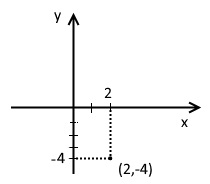
\includegraphics{./chapters/preliminares/imgs/Eixos}
\end{center}
\end{exemplo}

\noindent O plano Cartesiano é representado por $\R^2$.

%\vspace{0.5cm}

\noindent \textbf{Grafico de uma função:} Seja $f$ uma função com domínio e contra domínio no conjunto dos números reais. Então o gráfico de $f$ é o seguinte subconjunto de $\R^2$,

$$\mathbf{graf}(f)=\{(x,f(x))\in \R^2 : x\in \D(f)\}.$$

\noindent  O gráfico da função fornece uma forma importante de representar esta função. O gráfico de uma função $f$ é
normalmente representado por uma curva no plano, a qual é obtida marcando no plano cartesiano os pontos que fazem
parte do $\mathbf{graf}(f)$.

\section{Funções de Primeiro Grau}

Uma função é chamada de \textit{função de primeiro grau} se é dada por uma fórmula do tipo $f(x)=ax+b$ onde $a$ e $b$ são
números reais fixos e $a$ é não nulo.

\begin{exemplo}
A função
$$\begin{array}{crcl}f:&\R&\rightarrow &\R \\ &x&\mapsto& 2x-1 \end{array}$$

é de primeiro grau.
\end{exemplo}

\noindent \textbf{Equação do Primeiro Grau:} Uma equação do primeiro grau é uma expressão matemática do tipo:
$$ax+b=c$$
onde $a,\ b$ e $c$ são números reais fixos com $a \not=0$ e $x$ é chamado  \textit{incógnita}. Resolver o sistema linear é
encontrar um valor real que após substituído na incógnita torna a equação verdadeira. Para resolver a equação do primeiro grau
aplicamos o método que consiste em isolar a incógnita de um dos lados da igualdade.
Para tando, toda operação aplicada a um dos lados da igualdade será aplicado também
ao outro lado mantendo a igualdade verdadeira.


\begin{exemplo} Vamos resolver o sistema linear $3x-4=1$:

$$\begin{array}{cc}

&3x-4=1\\
\Leftrightarrow& 3x-4 \ (+4)=1\  (+4)\\
\Leftrightarrow& 3x=5\\
\Leftrightarrow& 3x\  (\div 3)=5\  (\div 3)\\
\Leftrightarrow&x=\displaystyle\frac{5}{3}.\end{array}$$

Portanto a solução da equação é $x=\frac{5}{3}.$
\end{exemplo}

\noindent\textbf{Gráfico da funçãoo de primeiro grau:} O gráfico da função de primeiro grau é
uma reta. Considere a função $f(x)=ax+b$. O número $a$ é o \textit{coeficiente ângular} da reta.
Se $a>0$ o gráfico de $f$ será uma reta
ascendente da esquerda para a direita. Se $a<0$ o gráfico de $f$ será uma reta descendente da esquerda para a direira.
Já o \textit{coeficiente linear}, $b$, indica o ponto onde esta reta cruza o eixo $y$.

\subsection{Aplicação: Custo, Lucro, Receita e Break Even Point}

Suponha o custo de produção de 1 unidade de determinado produto é constante e igual a $c_1$ (reais, dólares, euros, etc), então o custo de produção de $x$ unidades será $c_1x$. Não obstante, existem alguns custos que são fixos, isto é, independem
da quantidade de unidades produzidas, como por exemplo aluguéis e salários. Denotaremos a soma de todos os custos fixos por $c_0$. Portanto o \textit{custo total} na produção de $x$ unidades
será  $C(x)=c_1x+c_0.$


A \textit{receita} é o valor total ganho pela empresa na venda de seus produtos. Se cada unidade do produto é vendida por $p_1$
a receita obtida na venda de $x$ unidades será $R(x)=p_1x$. O \textit{lucro} obtido na venda de $x$ unidades é dado por $L(x)=R(x)-C(x)$.

\noindent\textit{Break Even Point:} é o ponto de equilíbrio entre custo total e receita, isto é $C(x)=R(x)$. No break even point o lucro será zero.

%\vspace{0.5cm}

\noindent\textbf{Graficamente:} Tanto o custo total quanto a receita são dados por retas. O break even point é o ponto onde estas retas se cruzam.


\begin{center}
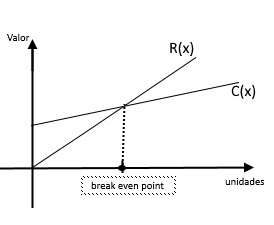
\includegraphics{./chapters/preliminares/imgs/breakeven}
\end{center}


\section{Sistemas Lineares}

Aqui trataremos apenas dos sistemas lineares de duas incógnitas. Para nós, sistema linear é um conjunto de equações
envolvendo duas incógnitas ( normalmente $x$ e $y$), em que cada equação possui a variável $x$ ou a variável $y$
com expoentes não maiores que 1. Mais precisamente, é uma expressão do tipo:
$$\left\{ \begin{array}{rcl}
a_{11}x+a_{12}y&=&b_1\\
a_{21}x+a_{22}y&=&b_2
\end{array}\right.$$

onde os coeficientes $a_{ij}$ e $b_{i}$, $i,j\in \{1,2\}$, são números reais fixos e as incógnitas são $x$ e $y$. Resolver o sistema é encontrar
um (ou mais ) valores para $x$ e $y$ que satisfaçam as duas equações simultaneamente.

Para resolver o sistema, são permitidos dois tipos de operações com as linhas do sistema:

\begin{itemize}
\item Multiplicação de uma linha por uma constante.
\item Somar duas linhas.
\end{itemize}

Estas operações são permitidas por que sua aplicação gera um novo sistema que possui as mesmas soluções do sistema original.

\begin{exemplo}Vamos resolver o sistema: $\left\{ \begin{array}{rcl}
2x-5y&=&1\\
x+y&=&2
\end{array}\right.$
\smallskip{}
\[
\left\{ \begin{alignedat}{1}2x-5y & =1\\
x+y & =2
\end{alignedat}
\xrightarrow{L_{1}\rightarrow L_{1}+5L_{2}}\right.\left\{ \begin{alignedat}{1}7x & =11\\
x+y & =2
\end{alignedat}
\xrightarrow{L_{1}\rightarrow\frac{1}{7}L_{2}}\right.\left\{ \begin{alignedat}{1}x & =\nicefrac{11}{7}\\
x+y & =2
\end{alignedat}
\right.
\]

\end{exemplo}

\noindent Substituindo o valor $x=\frac{11}{7}$ na segunda equação obtemos o valor $y=\frac{3}{7}$. Você pode verificar que esta é uma solução
substituindo os valores encontrados para $x$ e $y$ nas equações originais e se certificando que esta solução de fato satisfaz as equações,
como queríamos.

\noindent\textbf{Classificação:} Um sistema linear pertence obrigatóriamente a uma das três categorias abaixo:
\begin{mybox} \begin{itemize}
\item Quando um sistema admite uma única solução ele é dito \textit{possível e determinado}.
\item Quando um sistema admite infinitas soluções ele é dito \textit{possível e indetermindo}.
\item Quando um sistema não possui solução ele é dito \textit{impossível}.
\end{itemize}
\end{mybox}

\begin{exemplo} Vamos tentar resolver o sistema: $\left\{ \begin{array}{rcl}
2x+2y&=&1\\
x+y&=&2
\end{array}\right.$
\smallskip{}
\[
\left\{ \begin{array}{rcl}
2x+2y&=&1\\
x+y&=&2
\end{array}\right. \xrightarrow[]{L_1\rightarrow \frac{1}{2}L_1}\left\{ \begin{array}{rcl}
x+y&=&\frac{1}{2}\\
x+y&=&2
\end{array}\right.
\]

Subtraindo a primeira equação da segunda equação, isto é, fazendo $L_2-L_1$, obtemos: $0=\frac{3}{2}$.
Chegamos a um absurdo. Logo o sistema é impossível.
\end{exemplo}


\begin{exemplo} Vamos tentar resolver o sistema: $\left\{ \begin{array}{rcl}
x+2y&=&1\\
2x+4y&=&2
\end{array}\right.$
\smallskip{}
\[
\left\{ \begin{array}{rcl}
x+2y&=&1\\
2x+4y&=&2
\end{array}\right. \xrightarrow[]{L_1\rightarrow \frac{1}{2}L_2}\left\{ \begin{array}{rcl}
x+2y&=&1\\
x+2y&=&1
\end{array}\right.
\]

Portanto, após operações elementares aplicadas à primeira linha obtemos a segunda equação do sistema. Portanto, as duas
equações do sistema são equivalentes, e possouem a mesma solução. Concluímos assim que qualquer ponto da reta $y=\frac{1}{2}-\frac{1}{2}x$
é solução do sistema linear. Logo este sistema possui infinitas soluções, sendo assim do tipo Possível e Indeterminado.
\end{exemplo}

\section{Funções Quadráticas}

Seja $f$ uma função real  da forma $f(x)=ax^2+bx+c$, onde $a$,$b$ e $c$ são números reais fixos, e $x$ é a variável. Uma tal $f$ é chamada \textit{função quadrática} ou
\textit{função do segundo grau}.

%\vspace{0.5cm}

\noindent\textbf{Equação do segundo grau:} É uma equação da forma $ax^2+bx+c=0$. Uma solução é um valor real $r$ tal que quando substituímos $x=r$ na equação, a igualdade é verdadeira. Uma equação
do segundo grau pode não ter solução, ter apenas uma solução ou ter duas soluções. Na resolução de uma equação do segundo grau, apenas uma destas três possibilidades ocorrerá. A solução é feita completando quadrados,
o que produz a fórmula de Bhaskara.



\begin{exemplo}
\begin{multicols}{2}
Vamos resolver a equação:

$$3x^2-5x+2=0$$

Dividindo os dois lados da equação por $3$:

$$x^2-\frac{5}{3}x+\frac{2}{3}=0$$

Vamos completar quadrados. Isto é, devemos encontrar $r$
 e $\Delta$ de modo que

\begin{equation}\label{quadrado}
0=x^2-\frac{5}{3}x+\frac{2}{3}=(x-r)^2+\Delta. \end{equation}

\columnbreak

\begin{myboxblue}
\begin{minipage}{7cm}
Um quadrado perfeito é uma expressão do tipo:
$$(x-r)^2=x^2-2rx+r^2.$$
Completar quadrados é manipular uma expressão
de modo a obter um quadrado perfeito. Como fazemos no exemplo
ao lado.
\end{minipage}
\end{myboxblue}
\end{multicols}

Agora, usando a expressão para quadrados perfeitos (ao lado), temos
\begin{equation}\label{bhaskara}
x^2 \fbox{-$\dfrac{5}{3}x$}+\underbrace{\dfrac{2}{3}}=x^2 \fbox{$-2rx$}+\underbrace{r^2+\Delta}.
\end{equation}

Comparando o coeficiente do termo de grau 1,
que aparece à esquerda e à direita chegamos a:
$-2r=-\frac{5}{3} \Rightarrow r=\frac{5}{6}$.
Ainda, na equação (\ref{bhaskara}) temos que
$$\Delta=\frac{2}{3}- \frac{25}{36}=-\frac{1}{36}$$

Logo, substituindo $r$ e $\Delta$ na equação (\ref{quadrado}):

$$0=x^2-\frac{5}{3}x+\frac{2}{3}=(x-\frac{5}{6})^2-\frac{1}{36}.$$

Portanto nosso problema é equivalente a encontrar as raízes de:

$$(x-\frac{5}{6})^2-\frac{1}{36}=0.$$

Ou seja,

$$(x-\frac{5}{6})^2=\frac{1}{36}.$$

Daí,

$$ x-\frac{5}{6}=\pm \frac{1}{6}.$$

Portanto as raízes são $x=\frac{2}{3}$ e $x=1$.
\end{exemplo}

O procedimento do exemplo acima pode ser usado para deduzir a fórmula de Bhaskara para encontrar
as raízes da equação do segundo grau.

%\vspace{0.5cm}

\begin{multicols}{2}

\noindent \textbf{Gráfico da função do segundo grau:}O gráfico de uma função do segundo grau é uma parábola. Considere a função
$f(x)=ax^2+bx+c$. Se $a>0$ o gráfico é uma parábola com concavidade para cima. Se $a<0$ o gráfico é uma parábola de concavidade para baixo. Os dois casos estão representados ao lado.

\columnbreak

%\vspace{1cm}

\begin{center}
\begin{tabular}{cc}

\includegraphics{./chapters/preliminares/imgs/SadHappy.jpg} & 
\includegraphics{./chapters/preliminares/imgs/Happy.jpg} \\
$a<0$ & $a>0$
\end{tabular}
\end{center}
\end{multicols}

\section{Funções Elementares}

%\vspace{0.5cm}

\noindent\textbf{Função polinomial ou polinômio:}  É uma função da forma:
\begin{equation}\label{polinomio}f(x)=a_nx^n+a_{n-1}x^{n-1}+\ldots+a_1x^{1}+a_0\end{equation}
onde os coeficientes $a_i,\ i=0,1,\ldots n$ são números reais fixos. O expoente da maior potência de $x$ é o \textit{grau} do polinômio $f(x)$.

\begin{center}\fbox{\begin{minipage}{16cm}
\noindent\textbf{ OBS.:}Quando não é feita uma restrição sobre o domínio de $f$ podemos admitir que o domínio é toda a reta real $\R$, uma vez que uma fórmula do tipo
\ref{polinomio} está bem definida para qualquer valor que seja atribuido à variável  $x$.\end{minipage}}
\end{center}

\begin{exemplo} Toda função de primeiro grau é um polinômio de grau 1 e toda função de segundo grau é um polinômio de grau 2.
\end{exemplo}

\begin{exemplo} A função abaixo é um polinômio de grau 5:

$$P(x)=x^5-3x^3+2x^2+x-5.$$
\end{exemplo}

\noindent\textbf{Função Racional:} É uma função cuja fórmula é dada pelo quociente de dois polinômios, ou seja:
\begin{equation}
f(x)=\displaystyle\frac{a_nx^n+a_{n-1}x^{n-1}+\ldots+a_1x^{1}+a_0}{b_nx^n+b_{n-1}x^{n-1}+\ldots+b_1x^{1}+b_0}.
\end{equation}

Aqui destacamos que em geral uma função racional não pode ter como domínio todo o conjunto dos números reais, uma vez que quando o denominador
( $b_nx^n+\ldots+b_0$)
tem uma raiz real, digamos $x=x_0$, o quociente não estará definido justamente para $x=x_0$. Isto ocorre porque a divisão por zero não
é permitida dentro do conjunto dos números reais.

\begin{exemplo} A função abaixo é uma função racional

$$f(x)=\displaystyle\frac{2x^3-x^2+1}{x^2-1}.$$
Note que neste caso o denominador se anula em $x=1$ e em $x=-1$. Portanto o maior domínio possível para esta função são os números reais
diferentes de $1$ e $-1$, isto é $\R\setminus \{1,-1\}$.
\end{exemplo}

\noindent\textbf{Funções dadas por Radicais:}  A função raíz n-ésima é a função inversa da função n-ésima potência desde que
se faça  uma restrição adequada no domínio desta última. Por exemplo, digamos que queremos calcular a raíz quarta de
16, que representamos $\sqrt[4]{16}$, isto é, queremos encontrar um número real $x$ que elevado a quarta potência
dá 16. Mais precisamente, queremos encontrar uma solução de:
$$x^4=16.$$
Acontece que esta equação possui duas soluções reais, a saber $2$ e $-2$. Por isso foi convencionado que o símbolo
$\sqrt[4]{16}$, se refere apenas à solução positiva da equação acima, isto é $\sqrt[4]{16}=2$ .
O mesmo vale para todas raízer de ordem par: $\sqrt[2]{\cdot }$, $\sqrt[4]{\cdot}$, $\sqrt[6]{\cdot}$, etc.
\begin{center}
\begin{minipage}{16cm}\fbox{\noindent\textbf{OBS.:} Raízes de ordem par apenas estão definidas para números não negativos.
}
\end{minipage}
\end{center}
\begin{exemplo} A função $$f(x)=\sqrt[3]{x}$$

  é uma fução radical definida para todo número real. Já a função $$g(x)= \sqrt{x}$$

está definida apenas para valores não negativos de $x$ ($x\geq 0$).
\end{exemplo}


\section{Proporções e Porcentagens.}

Duas grandezas $x$ e $y$ são \textit{proporcionais} se existe uma constante não nula $k\in \mbox{R}\setminus \{0\}$ tal que $$y=kx.$$ Note que é um caso particular de função do primeiro grau, onde o coeficiente linear é zero.

Duas grandezas $x$ e $y$ são \textit{inversamente proporcionais} se existe uma constante não nula $k$ tal que $$y=k\frac{1}{x}.$$ Note que neste caso $y$ é proporcional ao inverso de $x$.

\clearpage

Apresentamos nos exemplos abaixo alguns problemas típicos envolvendo proporcionalidade.

\begin{exemplo} Em uma fabrica de camisetas, 10 trabalhadores produzem 160 camisetas por dia. Quantos trabalhadores serão necessários para produzir 240 camisetas por dia?

Presume-se que a quantidade de camisetas  produzida diariamente será proporcional ao número de trabalhadores. Desta forma,
se o número de camisetas produzidos por hora é $y$, e o número de fincionários é $x$, devemos encontrar a constante de proporcionalidade $k$ de modo que
\begin{equation}\label{proporção}y=kx.\end{equation}
O problema fornece a informação de que quando $x=10$ temos que $y=160$. Substituindo estes valores na equação acima, concluímos que $k=16$. Portanto, se $y=240$ temos pela equação (\ref{proporção}),

$$240= 16x\Rightarrow x=15.$$

Portanto serão necessários 15 funcionários para que se produza 240 camisetas por dia.
\end{exemplo}

\begin{exemplo} Uma torneira despeja água em um tanque com vasão constante de 10 litros por hora e consegue encher completamente este tanque em 3 horas. Uma segunda torneira de vasão 5 litros por hora é acrescentada e despeja sobre o mesmo tanque. Em quanto tempo as duas torneiras juntas encherão o tanque?

Naturalmente a vasão $V$ é inversamente proporcional ao tempo $T$ necessário para encher o tanque. Assim,

$$T=\frac{k}{V}.$$

Sabemos que se $V=10$ teremos $T=3$. Logo, $k=30$. Portanto, usando este valor de $k$, concluímos que o tempo necessário será de $2\ h$ quando a vasão for  $15\  l/h$ ( com as duas torneiras abertas).

\end{exemplo}



\noindent\textbf{Porcentagem:} Porcentagem é uma forma de comparar grandezas $x$ e$ y$ de mesma natureza (horas com horas, metros com metros, litros com litros, dólares com dólares etc).  Por exemplo, dizemos que $y$ é 5 \textit{por cento} de $x$ e representamos $5\%$  se $y/x=5/100$. Dizemos que $y$ é $17\%$ de $x$  se $y/x=17/100=0,17$, e assim por diante. Neste caso
o valor da porcentagem nos diz quantas unidades de $y$ teremos quando tivermos $100$ unidades de $x$.

\begin{exemplo} Em janeiro de 2016 a Barragem de Sobradinho dispunha de $3,5\%$ do seu volume útil para geração de energia elétrica.
Desta forma, considerando que o volume útil da barragem é de 28 bilhões de litros, temos que o volume útil disponível nesta data era de

$$V=0,034\times28\times10^9=9,52\times10^8 \ l.$$
\end{exemplo}

Porcentagens são comunmente usadas para comparação de quantidades.  No exemplo acima o valor $3,4\%$ significa que
para cada 100 litros da capacidade útil do reservatório, apenas 3,4 litros estavam disponíveis na data a que a informação se refere.

\begin{secaoexercicio}

\begin{xca} Determine se a relação expressa em cada um dos seguintes itens é uma função. Indique quando a função for injetiva, sobrejetiva ou bijetiva.

\begin{enumerate}[(a)]
\item A relação entre os conjuntos $A=\{1,2,3,4\}$ e $B=\{2,4,6,8\}$ dada por
$$\begin{array}{crcl}
f:&A&\rightarrow&B\\
&1&\mapsto&2\\
&2&\mapsto&4\\
&3&\mapsto&6\\
&4&\mapsto&8
\end{array}$$

\item A relação dada pelo gráfico abaixo:

\begin{center}
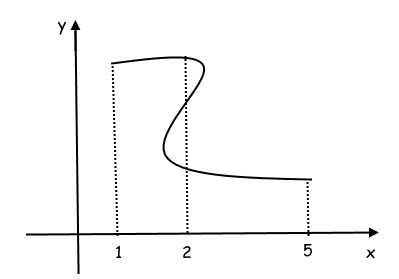
\includegraphics[scale=0.8]{./chapters/preliminares/imgs/naofuncao}
\end{center}

\item A relação
$$\begin{array}{crcl}
P:&\mathbf{R}&\rightarrow& \mathbf{R} \\
&x&\mapsto& x^2\end{array}$$
\end{enumerate}

\end{xca}

\begin{xca}  Resolva a equação, se houver solução:
\begin{colexercicio}{3}
\item $7x-2=1$
\item $4x-3=3$
\item $x^2+3x-4=0$
\item $2x^2-2x+\frac{1}{2}=0$
\item $x^2+2x+10=0$
\item $x^6+7x^3-8=0$
\item $-x^4+x^2+2=0$ (Dica: Use a substituição $y=x^2$)
\end{colexercicio}
\end{xca}

\begin{xca} Resolva o sistema linear, clssificando-o como possuindo solução única, infinitas soluções,
 ou mostre que o sistema não possui solução:
\begin{colexercicio}{3}
\item
$\left\{\begin{array}{c}
2x-5=0\\
x+y=1
\end{array}\right.$
\item
$\left\{\begin{array}{c}
x-2y=1\\
x-2y=2
\end{array}\right.$
\item
$\left\{\begin{array}{c}
3x+3y=3\\
2x-y=\frac{1}{2}
\end{array}\right.$
\item
$\left\{\begin{array}{c}
x+y=2\\
-x-y=1
\end{array}\right.$
\item
$\left\{\begin{array}{c}
5x+5y=10\\
-x-y=-2
\end{array}\right.$
\end{colexercicio}
\end{xca}
\end{secaoexercicio}
